\documentclass{article}


\usepackage{arxiv}

\usepackage[utf8]{inputenc} % allow utf-8 input
\usepackage[T1]{fontenc}    % use 8-bit T1 fonts
\usepackage{hyperref}       % hyperlinks
\usepackage{url}            % simple URL typesetting
\usepackage{booktabs}       % professional-quality tables
\usepackage{amsfonts}       % blackboard math symbols
\usepackage{nicefrac}       % compact symbols for 1/2, etc.
\usepackage{microtype}      % microtypography
\usepackage{lipsum}		% Can be removed after putting your text content

\usepackage[toc,page]{appendix}
\usepackage{amsmath}
\usepackage[ruled ]{algorithm2e}
\usepackage{tikz}
\usetikzlibrary{fit,positioning,arrows,automata,calc}
\tikzset{
	main/.style={circle, minimum size = 5mm, thick, draw =black!80, node distance = 15mm},
	invis/.style={circle, minimum size = 10mm, thick,  node distance = 15mm},
	connect/.style={-latex, thick},
	box/.style={rectangle, draw=black!100}
}

\title{Bachelor Project Report: \\ Multi-Object-Pose-Tracking on Point Detections}

%\date{September 9, 1985}	% Here you can change the date presented in the paper title
%\date{} 					% Or removing it

\author{
  Simon Giebenhain\thanks{The work was done as a Bachelors Project supervised by Prof. Bastian Goldlücke} \\
  Department of Computer Science\\
  University of Constance\\
  \texttt{simon.giebenhain@uni-konstanz.de} \\
}

\begin{document}
\maketitle

\begin{abstract}
%TODO
\end{abstract}


% keywords can be removed
%\keywords{First keyword \and Second keyword \and More}


\section{Introduction}


\subsection{Multi-Object Tracking}

Multiple Object Tracking (MOT), also known as Multi-Target Tracking, refers to the task of identifying and maintaining the identities of objects of interest over time. Usually MOT is performed on video data. Its most common applications are sports tracking, tracking of pedestrians and other traffic participants for surveillance purposes or autonomous driving. Despite the fact these applications are of particular interest for the industry, MOT remains a challenging task and an interesting research topic.


\subsection{The Specific Task at Hand}

The methods presented in this paper are tailored towards MOT on specific 3d bird trajectories. Next to the location, the orientation in three-dimensional space of the birds are being tracked. The data is described in detail in \ref{data_setup} and \ref{data_noise}.\\
This work particularly aims at building a foundation for analyzing the collective behaviour of birds at the department for Collective Behaviour from the Max Planck Institute and the University of Konstanz. The research group is using the VICON Tracker 3 system %TODO cite
to record the trajectories of multiple birds at once. However the acquired trajectories have a lot of holes, especially when the birds are moving. This work builds coherent 3d trajectories from unlabelled 3d detections. Further details are given in the section \ref{data_setup}.\\
For the behaviour analysis ID-switches are fatal. Therefore my approaches take special care of maintaining the identities of birds without switching them.



\subsection{Data Capturing Setup}
\label{data_setup}
% markers humanly designed, room for improvement
%TODO cite vogelwarte(https://de.wikipedia.org/wiki/Vogelwarte_Radolfzell) and VICON (https://www.vicon.com/software/tracker/)


%TODO marker setup 

It is important to understand the source of the data, as this information needs to be taken into account when designing a tracking algorithm.\\
The data was captured in inside of a large barn %TODO citation
with a 2D array of infrared cameras filming downwards from above. Each bird is equipped with a tiny backpack which has space for 4 infrared reflecting markers, positioned in a unique pattern. There can be elevations on the backpack, meaning that the specified pattern can be three-dimensional. Using these patterns enables to predict the orientation of the birds as well. These patterns are handcrafted. An analysis of the performance of the patterns could lead to insights, which allow for the design of better patterns. However such proceedings are out of scope for this work and may be subject to future research if need be.
%TODO rework pattern section above

The aforementioned infrared cameras feed information directly to the VICON Tracker3 system, which puts all detections into a unified three-dimensional coordinate system.  Although the room was painted, such that a minimal amount of infrared light gets reflected from anything else than the infrared markers, there is still a substantial amount of false positive (FPs) detections. Similarly there are lots of false negatives (FNs), especially when the birds are moving and occluding the markers with their wings. Some more details on the noise in the data is given in \ref{data_noise}.

%TODO: look at pigeon results, compare to starlings
 Tracker3 was specifically designed to operated on 3d detections from multiple infrared cameras. However the FN level is too high and the results of the Tracker3 are heavily compromised. As a result the output of the Tracker3 loses a majority of the tracks when the birds are moving.\\
 Hence this work is not utilizing the tracking results of the Tracker, but merely the detections over time in a unified three-dimensional coordinate system. The Tracker3 has a high accuracy at determining the 3d position of the markers, due to the multitude of cameras. For this reason this work assumes that the noise level (deviation of 3d detection to actual 3d position of marker) is very low.

\subsection{Exploring the Data}
\label{data_noise}
% e.g. fps
% different kind of noise present
% Unfortunately no ground truth to evaluate results, other than simulated data

As stated in the previous sections there is a lot of noise in the data. In this section I want to provide evidence for that claim...



\section{Related Work}
% research focuses on pedestrians,  and visual similarity, pose is uncommon, solely position no rotation
% reference 3D-Kalmanfilter paper to support choice of Klaman Filter
% check tracking the trackers and summarize some common approaches

% MILAN_RNN tries to tackle the problems in a unified framework
% Cite some interesting other appraoches


MOT is partly so challenging, because of the great variety of information present. Usually scenes are very busy, there can be an arbitrary number of objects of interest present and the camera position can change. As a result most approaches follow a \emph{tracking-by-detection} scheme, where an object detector locates objects of interest in each frame. This way the algorithm can focus on the information around the detected objects and discard information which seems irrelevant. The challenge is then to assign the detections to the tracks. This procedure is called \emph{detection to track assignment} and is the most crucial point of modern MOT algorithms. \\
This work also follows a \emph{tracking-by-detection} scheme, since the only available data are the 3d detections from the infrared cameras.

%TODO I should explain tracking by detection
Despite the great success of deep learning in most computer vision tasks over the past years, deep learning is only slowly improving MOT methods. \cite{milan_rnn_tracking} reason why applying deep learning to MOT is far from trivial. In MOT the tracked states are continuous, whereas the detection-to-track-assignment is a discrete assignment problem. The number of tracked objects is arbitrary and death and birth of tracks have to be handled. 

%TODO: look at popular papers
%TODO: also cite 3d Kalman Filter paper
Therefore the focus usually lies on constructing a similarity measure which incorporates visual appearance effectively...%TODO maybe link with following paragraph and move that paragraph up

\subsection{Differences to other works}
%TODO bird and death, we know how many birds in each scene, 

Most of the MOT literature focuses on tracking pedestrians, as surveillance and autonomous driving are two industry applications for MOT which drive research. Additionally the majority of research uses visual appearance features in order to make the \emph{detection to track assignment}. They do so for good reason, as \cite{tracking_the_trackers} found that the most defining feature of the best performing models on the MOT benchmarks is a good affinity measure using appearance features.

My task differs substantially from the majority of modern approaches to MOT. The methods presented here use no visual data and the usual \emph{detection to track assignment} is not sufficient to obtain good tracks. Since each bird has 4 markers, an exact \emph{detection to marker assignment} is necessary, especially to estimate the orientation well. \\
This task is complicated by a high rate of FPs and an even higher rate of FNs in the detections of the VICON system. 

The difficulties of my task deviate from the difficulties tackled in research. In the literature the main focus lies on modeling affinity in order to solve the \emph{detection to track assignment}. Clearly visual appearance is the richest source of information to that regard. Usually a strong affinity model is needed when working on detections in crowded scenes which are heavily troubled by occlusion. For this reason there is little research working on mere point detections.\\
In the setup presented here detections are three-dimensional and have a very high precision. This resolves occlusion problems and hence the \emph{detection to track assignment} is feasible in most cases, even when only incorporating proximity on predicted locations from a simple motion model, as shown in \ref{results_kalman_filter}. There are, however, two challenges remaining:
First, the \emph{detection to marker assignment} or identifying markers as FPs. A correct detection to marker assignment is crucial, in order to accurately predict the orientation, but especially challenging when less than 3 markers are detected or when FPs could not be identified. The problem becomes worse when the birds are moving the detection quality deteriorates for multiple consecutive frames.
Second, maintaining tracks over periods with no detections at all. In the most extreme cases predicting a correct orientation is almost impossible, but this can be tolerated. What is crucial in these situations is to maintain a good position estimation for several steps into the future in order to maintain the track as soon as a single detection reappears again. Doing so is especially important because initializing new tracks has to be done with extreme precaution, since ID-switches are not tolerated and it is important to identify the pattern in order to assign the new track to one of the birds. FPs are frequent and with no prior information about the position of a bird it becomes difficult to distinguish between FPs and TPs. Therefore it is important to have 4 true positive detections which match  the pattern of a missing birds exactly. Sometimes it can take hundreds of steps for such an occasion to occur. Therefore losing a track is very costly. %TODO find examples and check if it is actually true
%TODO If I extend createNewTrack() to work with 3 dets, make sure to update text

\section{My Approaches}

I followed two major approaches to solve the MOT problem, a classical Kalman Filter approach and a modern Deep Learning approach. The Kalman Filter(KF) is a very well known method across many different fields and seems like an obvious choice for tracking problems. The Kalman Filter is an algorithm that aims at uncovering some desired system state over time, by only seeing noisy measurements of some parts of the system. Due to the general formulation of the KF, it can be applied to lots of different scenarios. Some of these are: navigation and control, robotics, computer vision and econometrics. It is also used in every smartphone to estimate the orientation of the phone from noisy measurements of a gyroscope and accelerometer and for estimating geo-location from noisy GPS measurements. \\%TODO citation
Despite its simplicity it often works well on noisy real world data and is definitely an interesting baseline for the problem at hand. This choice is further supported by the work of \cite{3d_kalman}, who applied a KF to 3d LiDAR detections of the KITTI dataset (\cite{kitti}) and achieved state-of-the-art results on the KITTI 3D MOT challenge. %TODO read paper

Building upon the experience form the KF approach, I am currently trying to design a Deep Learning get better results. Another solution could be to help the KF at critical points with a Neural Network. %TODO complete paragraph, once I make progress

%TODO maybe notation section

%TODO also cite work of KF for orentation estimation somewhere



\subsection{Kalman Filter Approach}
\label{kalman_filter_approach}

%TODO: where should I explain the KF? in appendix? or nowhere and just go with notation
%TODO: read Computer Vision Book about KF, that I can even cite!

%TODO: section for how to arrive at initial guess???



%TODO explain how to get from single KF to MOT!!!


%TODO: Write two sentences about how I modeled the KF/system.
This approach models the dynamics of each bird with a separate KF and handles MOT with a set of heuristics and the Hungarian Algorithm (HA). %TODO citation.
The algorithm is described in the following: \\

\begin{figure}[!htbp]
	\begin{center}
	\includegraphics[scale=0.2]{img/flow_chart.png}
	\caption{ \textbf{Information flow through the KF-MOT architecture} - 
		(1) Each KF predicts location and orientation for frame $t$. (2) \& (3) The detections of frame $t$ are associated with the predicted positions. (4) The assignment is used to correct the KF predictions. (5) The active tracks are updated with the corrected predictions. (5) \& (6) The track management unit gets informed which tracks where unassigned and decides whether to discontinue the track or not. (7) \& (8) The track management unit gets all unassigned detections. If it detects the pattern of a untracked bird, a new track is initialized. }
	\label{flow_chart}
\end{center}
\end{figure}



\subsubsection{Defining the Domain Specific Kalman Filter}

\begin{figure}[!h]
	\centering
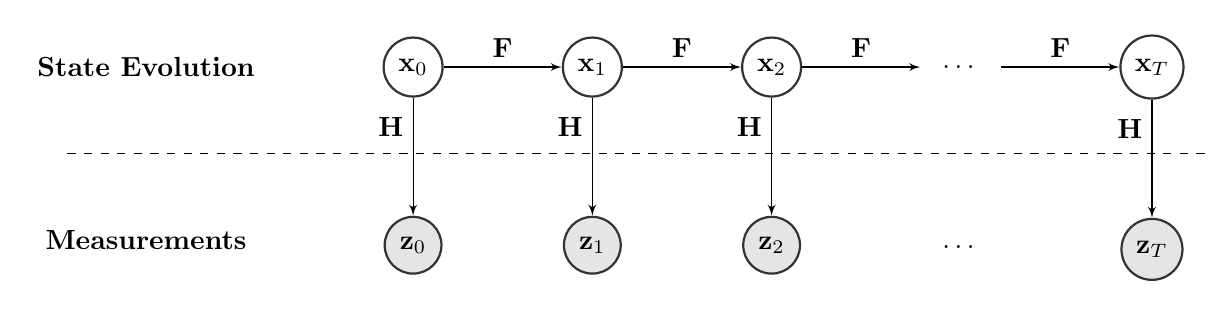
\begin{tikzpicture}[edge/.style = {->,> = latex'}]
\node[box,draw=white!100] (Latent) {\textbf{State Evolution}};
\node[main] (L1) [right=of Latent] {$\mathbf{x}_0$};
\node[main] (L2) [right=of L1] {$\mathbf{x}_1$};
\node[main] (L3) [right=of L2] {$\mathbf{x}_2$};
\node[invis] (L4) [right=of L3] {};
\node[main] (Lt) [right=of L4] {$\mathbf{x}_T$};
\node[main,fill=black!10] (O1) [below=of L1] {$\mathbf{z}_0$};
\node[main,fill=black!10] (O2) [below=of L2] {$\mathbf{z}_1$};
\node[main,fill=black!10] (O3) [below=of L3] {$\mathbf{z}_2$};
\node[invis] (04) [below=of L4] {};
\node[main,fill=black!10] (Ot) [below=of Lt] {$\mathbf{z}_T$};
\node[box,draw=white!100, below=of Latent, yshift=-7mm] (Observed) {\textbf{Measurements}};
\path (L3) to node {\dots} (Lt);
\draw[edge] (L1) to node[above] {$\mathbf{F}$} (L2);
\draw[edge] (L2) to node[above] {$\mathbf{F}$} (L3);
\draw[edge] (L3) to node[above] {$\mathbf{F}$} (L4);
\draw[edge] (L4) to node[above] {$\mathbf{F}$} (Lt);
\path (O3) to node {\dots} (Ot);
\draw[edge] (L1) to node[near start, left] {$\mathbf{H}$} (O1);
\draw[edge] (L2) to node[near start, left] {$\mathbf{H}$} (O2);
\draw[edge] (L3) to node[near start, left] {$\mathbf{H}$} (O3);
\draw[edge] (Lt) to node[near start, left] {$\mathbf{H}$} (Ot);

% draw the dashed line
\draw [dashed, shorten >=-1cm, shorten <=-1cm]
($(Latent)!0.5!(Observed)$) coordinate (a) -- ($(Lt)!(a)!(Ot)$);
\end{tikzpicture}
\caption{\textbf{The KF as a Graphical Model}}
\end{figure}

This section models the process described in section \ref{data_noise} as a Kalman Filter. The observations $\mathbf{z}_t$ are infrared detections, which are ideally four 3d points. Meaning that $\mathbf{z}_t \in \mathbb{R}^{12}$. However due to FPs and FNs this is not always the case. How these cases are handled is described in \ref{heuristics}. For now let's assume  $\mathbf{z}_t \in \mathbb{R}^{12}$. \\
The corresponding state $\mathbf{x}_t)$ holds the quantities to be estimated, which are the current position, $\mathbf{p}_t = (p_x, p_y, p_z)^T \in \mathbb{R}^4$ and orientation, $\mathbf{q}_t=(q_w, q_x, q_y, q_z)^T \in \mathbb{R}^4$ expressed as a quaternion, %TODO where to explain quaternions? 
as well as the current velocity, $\mathbf{v}_t=(v_x, v_y, v_z) \in \mathbb{R}^3$. This that this Kalman Filter assumes a constant velocity model for the position estimation and a brownian motion model for the orientation estimation. %TODO explain why I chose so, and google if there are better alternatives.

The state is $\mathbf{x}_t = (p_x, p_y, p_z, v_x, v_y, v_z, q_w, q_x, q_y, q_z)^T$.
The linear state transition function is 

$F =
\begin{pmatrix}
1 & 0 & 0 & 1 & 0 & 0 & 0 & 0 & 0 & 0 \\
0 & 1 & 0 & 0 & 1 & 0 & 0 & 0 & 0 & 0 \\
0 & 0 & 1 & 0 & 0 & 1 & 0 & 0 & 0 & 0 \\
0 & 0 & 0 & 1 & 0 & 0 & 0 & 0 & 0 & 0 \\
0 & 0 & 0 & 0 & 1 & 0 & 0 & 0 & 0 & 0 \\
0 & 0 & 0 & 0 & 0 & 1 & 0 & 0 & 0 & 0 \\
0 & 0 & 0 & 0 & 0 & 0 & 1 & 0 & 0 & 0 \\
0 & 0 & 0 & 0 & 0 & 0 & 0 & 1 & 0 & 0 \\
0 & 0 & 0 & 0 & 0 & 0 & 0 & 0 & 1 & 0 \\
0 & 0 & 0 & 0 & 0 & 0 & 0 & 0 & 0 & 1 \\
\end{pmatrix}
$
$F$ models the dynamics of a constant velocity model for the position estimation and a brownian motion model for the orientation estimation. 

The measurement function $H$ mapping from state space to measurement space is unfortunately not linear anymore. The problem is the inherent non-linearity of rotations. Whereas a fixed rotation is a linear operation, the rotation becomes non-linear when the parameters describing the rotation are seen as variables, which is exactly the case here. \\
The non-linear version of the measurement function $h: \mathbb{R}^{10} \rightarrow \mathbb{R}^{12}, (\mathbf{p}, \mathbf{v}, \mathbf{q})^T \mapsto \text{Rot}(\mathbf{q})\mathbf{p}$, where $\text{Rot}(\mathbf{q})$ denotes the rotation matrix, which describes the same rotation as the quaternion $\mathbf{q}$. See appendix \ref{quat_to_mat} for details. \\
The Extended Kalman Filter (EKF) is a simple extension of the simple KF, which can handle non-linear state-transition functions and non-linear measurement functions, by approximating them with their Jacobians. The Jacobian is locally the best linear approximation to a non-linear function. This approximation can deteriorate the performance of the EKF, when very non-linear functions are used. %TODO investigate measurement function H and state why linear approximation is OK in this case.

$Q_t$ is the covariance matrix of the process noise and $R_t$ is the covariance matrix for the measurement noise.

In total this amounts to the following equations describing the system:

$\mathbf{x}_{t+1} = F\mathbf{x}_t + \mathbf{w}_t$, where $\mathbf{w}_t \sim \mathcal{N}(0, Q_t)$.

$\mathbf{z}_{t} = H\mathbf{x}_t + \mathbf{v}_t$, where $\mathbf{v}_t \sim \mathcal{N}(0, R_t)$.


\subsubsection{Data Association}
\label{heuristics}
% I applied a set of heuristics in order to tackle the data specific difficulties. as described in ref sec 2.2
As explained in \ref{kalman_filter_approach}, this is the key tasks to be performed in MOT. This component enables MOT by stringing together all the independent EKFs. The method described in the following relies heavily on heuristics and hyper-parameters. The choices made were not extensively tested. In the future this task could be done with a neural network, which works better on a large variety of possible scenarios than these handcrafted rules.

\paragraph{Detection to Track Assignment} 
The first step is to do the detection to \emph{track} assignment. This is just a small preprocessing step to make the \emph{detetion to marker assignment} easier. The optimal assignment is calculated with a version of the Hungarian Algorithm, which additionally allows unassigned tracks and unassigned detections. The assignment costs are based on the distances of the predicted marker locations to the detections. The cost of not assigning a detection to any track and not assigning any detection to a track is set to 50. As the pairwise distances of the points in a pattern are roughly ranging between 15 and 50, this is a bit generous and will tend to sometimes assign FPs to a track if there are some FNs. Experiments showed that setting a lower value, will lead the system to lose tracks, when the constant velocity model of the Kalman Filter fails to predict a precise position for the next frame. Setting the cost for non-assignments too high will sometimes cause multiple FPs assigned to a track. This renders the algorithm explained in the next paragraph inefficient, since it considers all permutations of the detections assigned to a single track.

\paragraph{Detection to Marker Assignment}
When there are 2 or less detections assigned to a track, there is not enough information to reason about the orientation of the pattern. Then the assignment to markers is solely based on the predicted marker locations, exactly as in the \emph{detection to track assignment}.\\
If there are 3 or more detections assigned to a track, the structure of these three detections can give clues about the orientation of the pattern. This case is handled with a simple brute-force method, which calculates costs for every possible detection to marker assignment. The costs are composed of 4 parts:
\begin{equation}
\begin{split}
 \text{cost(pattern, det)} \quad = \quad  ~ \text{MSE}\left(\texttt{pdist}(\text{pattern}) - \texttt{pdist}(\text{det}) \right)  \qquad \qquad \qquad \qquad \qquad \quad \\
  +\quad \lambda \cdot \text{MSE}\left( \texttt{pangles}(\text{pattern}) - \texttt{pangles}(\text{det}) \right) \qquad \qquad \qquad ~~ \\
  +\quad \text{MSE}\left(\texttt{rot}(\text{pattern},\hat{q}_t) - det\right) \quad \qquad \qquad \qquad \qquad \qquad \quad ~\\
  +\quad \texttt{costOfNonAssignment} \cdot \#(\text{non-assignments}) \quad \qquad \qquad \quad
\end{split}
\end{equation}

, where \emph{pattern} are the 4 markers ordered by one of the permutations, \emph{det} are the detections, \texttt{pdist} and \texttt{pangles} are functions calculating the all pairwise distances and angles respectively,  \texttt{rot} rotates pattern as described by $\hat{q}_t$, and $\#(\text{non-assignments})$ are the number of detections which were not assigned to a marker. The permutations are calculated such that it is possible to not assign all but 3 markers. $\lambda$ and \texttt{costOfNonAssignment} are two more hyperparameters to balance the influences of the parts.

\subsubsection{Track Management Unit}
This part of the system reasons about the death and birth of tracks. %TODO new paragraph for death as well?
The death of tracks is governed by one rule  only. This rule removes track which were not assigned any detections for more than \texttt{invisibleForTooLong=20} many frames.

\paragraph{Creating New Tracks} 
Since ID-switches are to be avoided, new tracks are only created if there are 4 detections that match a pattern of an untracked bird close to exact. The unassigned detections are clustered based on distances. The matching of such a cluster detections with a pattern is done with the method developed in \cite{umeyama}. This method finds the optimal (with respect to least square error) rotation, translation and scaling transformations to transform one set of m-dimensional points to match another set. As there can be many such clusters and untracked bird, the Hungarian Algorithm is applied once more. For each pair of cluster and pattern, the cost is calculated as the mean squared error output by the Umeyama matching. There is another handcrafted cost of non assigned, which is set very low in order to only create new tracks, when the detections match a pattern very close. The translation vector is used as initial position of the track and the rotation matrix is converted to a quaternion and used as initial orientation.




\subsection{Deep Learning Approach}
% Differences to common models
\subsubsection{Lack of Training Data}

\subsubsection{Own Model Architecture}

\subsubsection{Training Details}

\subsubsection{How to Improve the Model}

\section{Results}


\subsection{Kalman Filter}
\label{results_kalman_filter}

\subsection{Deep Learning Approach}

\section{Future Work}
%TODO explain detection to track assignemnt in related work
% TODO explain detecton to marker assignemnt later on!
%TODO nochmal proof readen, shr sloppy geschrieben
The solid performance of the Kalman Filter approach shows that a simple position prediction method, like a constant velocity model, is enough in most cases to maintain the tracks over time and inhibit ID-switches. Since the position of birds does not change drastically within a single time step, the detection to track assignment, which is the most critical step in MOT, is relatively easy. However the exact detection to marker assignment is harder already. However an exact detection to marker assignment is not strictly necessary, since error introduced by such are quite small. \\
There are however two major difficulties that remain:
First, orientation estimation is especially challenging because small mistakes in the detection to marker assignment or an undetected FP can completely disrupt the estimation. This problem could be tackled with better heuristics Since coming up with viable heuristics can be very tedious, a Neural Network could be trained to handle the detection to marker assignment. Such an approach will be subject of future research.\\
Secondly long term predictions are are required to fill gaps in cases with no or very few detections for multiple consecutive frames. As \cite{tracking_the_trackers} found, most MOT algorithms increase the FN rate, instead of decreasing it by filling in gaps. This leads to the conclusion that \emph{trajectory prediction literature} seems more promising than \emph{MOT literature} to tackle the problem at hand. Since even the simple constant velocity motion model of the EKF was sufficient to produce good position estimation and inhibit any ID-switches, it seems reasonable to disregard the tracking of multiple objects, focus on good trajectory prediction and obtain MOT by the Hungarian Algorithm and simple heuristics to manage the birth and death of tracks.

\section{Summary}

\begin{figure}[ht]
	\centering
	\begin{minipage}{.7\linewidth}
		%TODO new names nlset{}
		
		\begin{algorithm}[H]
			\DontPrintSemicolon
			\KwData{$G=(X,U)$ such that $G^{tc}$ is an order.} %TODO
			\KwResult{$G’=(X,V)$ with $V\subseteq U$ such that $G’^{tc}$ is an %TODO
				interval order.}
			\Begin{
				\nl Initialize tracks \;
				\For{$d\in D$}{
					\nlset{predict()} KF predict step \; %TODO for eacvh active track do predict
					\nlset{detectionToMarkerAssignment()} Assign detections to markers\; \label{detection_to_marker_assignment} %TODO details later
					\nlset{correct()} KF correct step \; % TODO fora each actove track correct()
					\nlset{deleteTracks()} Decide if tracks were lost \; %TODO give details here
					\nlset{createTrcks()} Create new tracks if pattern could be found in unassigned detections \; %TODO details later
				}
			}
			\caption{MOT with multiple KFs} %TODO
			
		\end{algorithm}
		
	\end{minipage}
\end{figure}

\bibliographystyle{apalike}  
\bibliography{references}

\begin{appendices}

\section{Quaternions}
\subsection{From Quaternions to Rotation Matrices}
\label{quat_to_mat}
% TODO


\end{appendices}


\end{document}
